\section{Evaluation}
We first present the experimental setups, then conduct an ablation study to
determine the proper prefix in PGG training, before our main 
results. More implementation details are in \apxref{sec:details}.

\subsection{Experimental Setup}
We implement our experiments on \textbf{SAMSum}~\cite{gliwa2019samsum}
and  \textbf{DialSumm}~\cite{chen-etal-2021-dialogsum}, whose statistics 
are listed in Table \ref{tab:sumdataset}. 
%Compression ratio equals SW divided by DW, 
%showing that summaries in DialSumm are more compressed than in SAMSum.



\begin{table}[th]
	\scriptsize
	\centering
	\begin{tabular}{p{0.8cm}rrrrr}
		\toprule[1pt]
		\textbf{Datasets}& \textbf{Variation} & \textbf{Train/Val/Test} & \textbf{IW} & \textbf{OW} & \textbf{CR} \\
		\midrule[1pt]
		\multirow{2}{*}{SAMSum}& DSum & 14,731/818/819 & 124.10 & 23.44 & 0.25\\
		&DialSent& 29,757/1,654  & 149.93 & 11.93 & 0.13\\
		\multirow{2}{*}{DialSumm} & DSum & 12,460/500/500 & 187.52 & 31.02 & 0.18 \\
		& DialSent&22,407/840  &214.00 & 17.78 & 0.10 \\
		\bottomrule[1pt]
	\end{tabular}
	\caption{Statistics of dialogue summarization datasets. IW, OW and CR represent the number of input words, the number of output words and compression ratio (OW/IW) respectively.}
	\label{tab:sumdataset}
\end{table}

We compare our method with these baselines.
\textbf{Lead-3} and \textbf{Longest-3} are simple rule-based 
baselines that extract the first or the longest $3$ utterances in 
a dialogue as the summary respectively. 
\textbf{PGN}~\cite{see2017get}, \textbf{Fast-Abs}~\cite{chen2018fast}, and \textbf{PEGASUS}~\cite{zhang2020pegasus} are well-known models for text summarization. \textbf{BART}~\cite{lewis2020bart} is a general PLM and performs well after fine-tuning.
\textbf{CODS}~\cite{wu-etal-2021-controllable}, \textbf{Multi-view}~\cite{chen2020multi} and \textbf{DialoBART}~\cite{feng-etal-2021-language} are the SOTA models designed for dialogue summarization.

We evaluate both automatically and by human.
For \textbf{automatic evaluation}, we use Rouge-1, 2, and L~\cite{lin2004rouge} 
F1-scores~\footnote{\url{https://pypi.org/project/py-rouge/}}. 
Following \citet{feng-etal-2021-language}, we adopt the same Rouge evaluation tool and compute between reference summaries and generated summaries. For DialSumm, we use maximum rouge scores among references for each sample.
For \textbf{human evaluation}, we three proficient English speakers to evaluate 100 
random samples from SAMSum.  
Each original dialogue and its reference summary are shown with generated summaries in a random order simultaneously. Showing summaries from different approaches together helps humans do comparisons between them.
Following \citet{chen2020multi} and \citet{liu2021coreference}, 
each summary is scored on the scale of $[2, 0, -2]$, where $2$ means concise 
and informative, $0$ means acceptable with minor errors, and $-2$ means 
unacceptable. The final scores are averaged among annotators.
We also ask human annotators to label the error types in the summary. 
We consider the following 4 error types:
\textbf{Mis}sing important contents, 
\textbf{Red}undant content, 
\textbf{Cor}eference mismatches, and
\textbf{Rea}soning error.
Rea and Cor concentrate on comparisons to the dialogue, 
and the rest two focus on comparisons to the reference. 
We determine the error for each case by majority voting, and count the errors of each model.

%\subsection{Results and Discussions}
%
%We present a comparison of different post-training approaches. Then, we do ablation studies for our best approach, PGG with DialSent. Finally, we compare it with state-of-the-art models. %with comprehensive analysis.
%

%\begin{table}
%	\small
%	\centering
%	\begin{tabular}{lccc}
%		\toprule[1pt]
%		\textbf{Models} & \textbf{Rouge-1} & \textbf{Rouge-2} & \textbf{Rouge-L} \\
%		\midrule[1pt]
%		\multicolumn{4}{l}{\textit{SAMSum}} \\
%		{BART} &52.06 &27.45 &48.89 \\
%		{DialIndirect} &  53.08&28.51  & \textbf{50.25} \\
%		{ExtSum} &  53.20& 28.26 & 49.80 \\
%		{ExtSumM} & 52.20 & 27.91 & 49.74   \\
%		{EntSent} & 51.82 & 27.43 & 49.19   \\
%		{ExtSentM} & 51.66 & 27.27 &  48.96  \\
%		{DSum} & 52.52&27.51 &49.03 \\
%		{DialSent} & \textbf{53.54} & \textbf{28.91} &  50.21 \\
%		
%		\midrule[1pt]
%		
%		\multicolumn{4}{l}{\textit{DialSumm}} \\
%		{BART} & 53.01&29.18 &51.34 \\
%		{DialIndirect} &  52.54&29.13  &51.68 \\
%		{ExtSum} & 51.83 & 27.92 &50.33  \\
%		{ExtSumM} & 52.29 & 27.72 & 50.09   \\
%		{EntSent} & 51.41 & 27.81 & 49.65   \\
%		{ExtSentM} & 52.46 & 28.86 & 51.36 \\
%		{DSum} & 53.27 & 28.64 & 51.69 \\
%		{DialSent} &\textbf{54.73} & \textbf{30.47}&  \textbf{53.46}  \\
%		\bottomrule[1pt]
%	\end{tabular}
%	\caption{Comparisons among different post-training approaches and fine-tuning-only BART baseline on dialogue summarization.}
%	\label{tab:rephrasing}
%\end{table}

%\subsection{Comparison on Post-training Approaches}\label{sec:posresult}
%
%The statistics of post-training datasets derived from SAMSum and DialSumm are shown in Table~\ref{tab:rephrasedatasets}. We compare the performances between different rephrasing approaches with these datasets of our two-stage approach with the fine-tuning-only BART. The results are shown in Table~\ref{tab:rephrasing}. 
%
%\begin{table}[th]
%	\small
%	\centering
%	\begin{tabular}{lrrrr}
%		\toprule[1pt]
%		\textbf{Datasets} & \textbf{Train/Val} & \textbf{IW} & \textbf{OW} & \textbf{CR} \\
%		\midrule[1pt]
%		\multicolumn{5}{l}{\textit{SAMSum}} \\
%%		{DialIndirect} & 14,731/818 & 124.10 & 157.41 & 1.31 \\
%%		{ExtSum} & 14,731/818 & 31.23 & 23.44 &0.94  \\
%%		{ExtSumM} & 14,731/818 & 66.09 &23.44 & 0.69 \\
%%		{EntSent} & 29,757/1,654 & 31.05 & 11.93 &0.68  \\
%%		{ExtSentM} & 29,757/1,654 & 46.45 & 11.93 & 0.60 \\
%		{DSum} & 14,731/818 & 124.10 & 23.44 & 0.25 \\
%		{DialSent} &29,757/1,654  & 149.93 & 11.93 & 0.13 \\
%		\midrule[1pt]
%		\multicolumn{5}{l}{\textit{DialSumm}} \\
%%		{DialIndirect} & 12,460/500 & 187.52 & 215.30 & 1.16 \\
%%		{ExtSum} & 12,460/500 & 44.43 & 30.02 &0.84 \\
%%		{ExtSumM} & 12,460/500 & 94.32 &31.02 &0.61  \\
%%		{EntSent} & 22,407/840 & 39.27 &17.78  &0.65  \\
%%		{ExtSentM} &22,407/840  &61.17  & 17.78 & 0.56 \\
%		{DSum} & 12,460/500 & 187.52 & 31.02 & 0.18 \\
%		{DialSent} &22,407/840  &214.00 & 17.78 & 0.10 \\
%		\bottomrule[1pt]
%	\end{tabular}
%	\caption{Statistics of constructed datasets. IW and OW refer to the number of words in the input and output of corresponding dataset.}
%	\label{tab:rephrasedatasets}
%\end{table}
%
%
%DialIndirect performs incredibly well on SAMSum. However, if we use the converted dialogue as input and directly fine-tune the original BART, the results are only 50.91/28.51/50.25 for Rouge-1/2/L.
%%, showing that such direct transformation doesn't help with the cross-format understanding. 
%It shows that when accompanied with the post-training stage, the model can learn relationships between speakers and utterances, and boundaries of utterances better than a direct transformation of dialogue inputs. 
%This rule-based transformation falls on DialSumm compared with BART baseline. More complicated rules may lead to better results, but such labored work is not what we are after. 
%
%The extraction-based methods fall behind the others. The modification to the algorithm tends to bring more noises than useful information to the input as the results drop mostly. 
%Besides, splitting the summary into sentences doesn't improve the results here.
%In a word, such hard extractions hurt the intricate discourse and coreference relations among utterances and are not suitable for cross-format data construction.
%
%DialSent with PGG task outperforms other methods and BART consistently across datasets, while DSum with PGG performs almost the same as BART.
%If we use DialSent data to augment the original DSum during fine-tuning, the results on SAMSum are 44.61/22.81/44.15 for Rouge-1/2/L respectively showing that the data in both datasets is not compatible. Thus, our approach is different from data augmentation.
%Overall, post-training with cross-format rephrasing intuition does help with dialogue summarization,
%


\subsection{Ablations Study}\label{sec:pggablation}
%
We conduct ablations to verify the effectiveness of post-training on DialSent with PGG, including post-training on DSum with PGG task (DSum-PGG), DSum with vanilla generation task (DSum-VG), and DialSent with vanilla generation task (DialSent-VG) in Table~\ref{tab:pggablation}.
The results of DSum-VG drop, indicating that fine-tuning for BART on DSum with early-stop is enough. Post-training with the same data and task leads to overfitting. 
%%overfit some expressions in summaries, so that Rouge-L increases.
%%DSum-PGG and DialSent-VG performs slightly better than BART. These two post-training methods are both more simple than dialogue summarization with multiple sentences and without guidance, acting as a preparation for fine-tuning.
DialSent-PGG performs best for two reasons. Compared with DialSent-VG, the prefix solves one-to-many mappings between a dialogue and summary sentences, so that the same dialogue can lead to different generations.
On the other hand, 
%%we can regard the ability of dialogue summarization into content selection and rephrasing of cross-format information. 
the prefix can manipulate the selection within a short sentence but is not strong enough to direct content in multiple sentences. Thus, DialSent-PGG learns more cross-format paraphrasing ability and performs better.
%
\begin{table}
	\scriptsize
	\centering
	\begin{tabular}{lccc}
		\toprule[1pt]
		\textbf{Models} & \textbf{Rouge-1} & \textbf{Rouge-2} & \textbf{Rouge-L} \\
		\midrule[1pt]
		\multicolumn{4}{l}{\textit{SAMSum}} \\
		%\textbf{BART}  &52.06 &27.45 &48.89  \\
		{DSum-VG} &51.48 &27.27 &49.45 \\
		{DSum-PGG} &52.52 &27.51 & 49.03\\
		{DialSent-VG} &52.16 &27.79 & 49.41\\
		{DialSent-PGG} &\textbf{53.54} &\textbf{28.91} &\textbf{50.21}\\
		\midrule[1pt]
		\multicolumn{4}{l}{\textit{DialSumm}} \\
		%\textbf{BART} &  53.01&29.18 &51.34  \\
		{DSum-VG} &53.15 &28.86 & 51.48\\
		{DSum-PGG} &53.27 &28.64 &51.69 \\
		{DialSent-VG} &52.99 & 29.14& 51.40\\
		{DialSent-PGG} &\textbf{54.73} & \textbf{30.47}&\textbf{53.46} \\
		\bottomrule[1pt]
	\end{tabular}
	\caption{Ablations on DialSent with PGG task.}
	\label{tab:pggablation}
\end{table}

\begin{table}[th]
	\scriptsize
	\centering
	\begin{tabular}{llll}
		\toprule[1pt]
		\textbf{Models} & \textbf{Rouge-1} & \textbf{Rouge-2} & \textbf{Rouge-L} \\
		\midrule[1pt] 
		\multicolumn{4}{l}{\textit{SAMSum}} \\
		{w/o} & 52.16 & 27.79& 49.41\\
		{const} & 51.71& 27.34&49.25 \\
		{random} & 52.32& 27.99&49.68 \\
		{Ling-Noun} &\textbf{53.54} & \textbf{28.91}&50.21\\
%		{Ling-Verb} &53.11 &28.35 &50.05 \\
%		{Ling-Subj} &52.90 &28.50 & \textbf{50.26}\\
%		{Ling-Root} &53.21 & 28.48&50.16 \\
		\midrule[1pt]
		\multicolumn{4}{l}{\textit{DialSumm}} \\
		{w/o} & 52.99& 29.14&51.40 \\
		{const} &53.29 &29.57 &52.10 \\
		{random} &53.82 & 29.88&52.43\\
%		{Ling-Noun} &53.37 & 29.60& 52.05\\
%		{Ling-Verb} &53.70 & 29.43&53.01 \\
%		{Ling-Subj} &52.17 & 28.54&50.78 \\
		{Ling-Root} &\textbf{54.73} & \textbf{30.47}&\textbf{53.46}\\
		\bottomrule[1pt]
	\end{tabular}
	\caption{Ablations on prefix designs for PGG.}
	\label{tab:prefixablation}
\end{table}

We try several choices of prefix length:
(1) \textbf{W/O}: without any prefix.
(2) \textbf{Const}: Constant length set to 2 and 3 for SAMSum and
DialSumm respectively, since a person's name is $1.69\pm0.69$ tokens long
on average~\footnote{DialSumm normalizes speaker names 
into ``\#Person1\#'' resulting in more tokens.}.
%summary start with a name and names can be tokenized to 
%$1.69\pm0.69$ tokens on average according to the datasets. So, we set the constant as $2$ and $3$ for SAMSum and DialSumm respectively
%Besides, ``\#'' is recognized as a single word by Spacy, which influences the pos tagging and dependency parsing accuracy. }.
(3) \textbf{Random}: set by uniform sampling from a range of numbers. 
We set the range to $1\sim3$ and $2\sim4$ for the two datasets respectively.
(4) \textbf{Ling}: using the validation set, we determined that Noun and Root 
are the best choice for the two datasets, respectively. In this way, the number of prefix tokens for SAMSum and DialSum are $1.90\pm1.10$ and $3.55\pm1.24$.
%We regard these different choices under Ling as the only hyper-parameter newly introduced in our approach.

In \tabref{tab:prefixablation}, Ling performs the best among these variants.
The actual linguistic feature to use may vary from dataset to dataset though.
The remaining experiments will be conducted using PGG-Ling.
%Without prefix, the same dialogue may lead to different sentences which may confuse the model on what to generate. 
%Const fails on cases where the output starts with stopwords. The prefix will not be informative enough to guide the model on what to rephrase. Random performs better because the same sample in different epochs may be assigned a different number of prefix tokens. %It can be regard as a data augmentation. 
%Const and Random are coarse without considering the output sentence specifically.
%
%In the contrary, linguistic features can provide more proper prefix tokens considering individual differences of samples. The performance of different features may be variant due to the accuracy of POS tagging and dependency parsing. For example, subj tags for sentences in DialSumm are poor due to special tokens for person names while the others are acceptable. 
%Overall, prefix tokens determined by linguistic tags lead to more promising results.

\begin{table}[th]
	\scriptsize
	\centering
	\begin{tabular}{lccc}
		\toprule[1pt]
		\textbf{Models} & \textbf{Rouge-1} & \textbf{Rouge-2} & \textbf{Rouge-L} \\
		\midrule[1pt]
		\multicolumn{4}{l}{\textit{SAMSum}} \\
		%\textbf{BART}  &52.06 &27.45 &48.89  \\
		{Lead-3} & 31.41& 8.68&30.38 \\
		{Longest-3} &32.46 &10.27 &29.92 \\
		{PGN} &40.08 &15.28 &36.63 \\
		{Fast-Abs} &41.95 &18.06 &39.23 \\
		{PEGASUS}& 50.50 & 27.23 & 49.32 \\
		{BART$^\dag$} &52.06 &27.45 &48.89 \\
		{CODS} &52.65 &27.84 &50.79 \\
		{Multi-view} & 53.42& 27.98& 49.97\\
		{DialoBART} &\textbf{53.70} &28.79 &\textbf{50.81} \\
		{DialSent-PGG$^\dag$} &\underline{53.54} &\textbf{\underline{28.91}} &\underline{50.21} \\
		\midrule[1pt]
		\multicolumn{4}{l}{\textit{DialSumm}} \\
		%\textbf{BART} &  53.01&29.18 &51.34  \\
		{Lead-3} &31.15 &10.08 &30.68\\
		{Longest-3} &27.00 &9.41 &25.31 \\
		{BART$^\dag$} & 53.01& 29.18& 51.34\\
		{DialoBART$^\dag$} &53.26 &29.58 &52.01 \\
		{DialSent-PGG$^\dag$} &\textbf{\underline{54.73}} &\textbf{\underline{30.47}} &\textbf{\underline{53.46}} \\
		\bottomrule[1pt]
	\end{tabular}
	\caption{Dialogue summarization results compared with baselines. $\dag$ represents the models implemented by ourselves. \underline{Underlined} scores are statistically significantly better than BART with $p<0.05$ based on t-test. }
	\label{tab:end2end}
\end{table}

\subsection{Comparison to SOTA Models}\label{sec:end2end}

%We compare our approach with baselines and the results are shown in Table~\ref{tab:end2end}. Most results for SAMSum are borrowed from~\cite{feng2021survey}. We implement the BART baseline and the state-of-the-art approach DialoBART on DialSumm for comparison.
%Rule-based baselines, i.e. Lead-3 and Longest-3, for dialogue summarization are not as good as for news summarization due to the format and discourse divergence between news and dialogues. 
%Models designed for news summarization also perform poorly on dialogue summarization, including PGN and Fast-Abs without pre-training and PEGASUS with pre-training for summarization on narrative texts.
%BART, which is pre-trained as a general language model, performs better. Further works injecting dialogue features based on BART achieve significant improvements, including CODS with intent, key phrase and segmentation, Multi-view with topic and stage segmentation, and DialoBART with keyword, redundancy and topic features. 
%All of these features are much harder to collect than our prefix tokens.
%CODS prefixes the intent and key phrase as summary sketch at the beginning of outputs, which are much harder to collect than our prefix tokens.
%FROST utilizes more simple features which appends recognized named entities in the input at the beginning of the output more informative summaries. It achieves limited improvements on dialogue summarization. 
\textbf{Automatic Evaluation:} 
Our model DialSent-PGG performs competitively against other models on 
SAMSum and significantly better than the peers on DialSumm. 
It improves 1.5 on Rouge scores over BART for both datasets, 
while DialoBART achieves less gains on DialSumm. 
Based on Table~\ref{tab:datasets}, DialSumm is a more difficult dataset 
with lower compression ratios. Our model performs better on samples 
with lower CR, i.e. more compressed samples, as shown in Figure~\ref{fig:cr}, thus differences 
between DialSent-PGG and DialoBART are more obvious on DialSumm. 
A simple case study is shown in Table~\ref{tab:case}.  
Multi-view faces the repetition problem as it takes the dialogue as 
input twice with two encoders. DialoBART has reasoning errors because 
it regards ``William'' as a keyword. DialSent-PGG instead generates a 
concise and correct summary. More cases are in \apxref{sec:cases}.

\begin{figure}
	\centering
	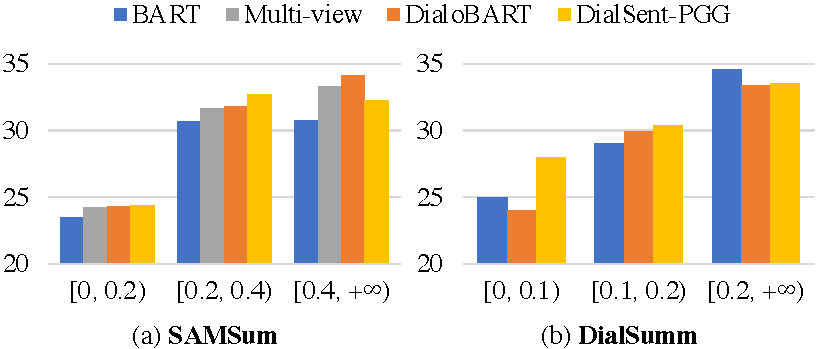
\includegraphics[scale=0.45]{compressionratio.pdf}
	\caption{Comparison for models on samples with different CR. X-axis represents the ranges for CR(\%). Y-axis is the Rouge-2 F1(\%).}
	\label{fig:cr}
\end{figure}

\begin{table}[th]
	\scriptsize
	\centering
	\begin{tabular}{lp{4.8cm}}
		\toprule[1pt]
		 {Dialogue}& \makecell[l]{William: are you still angry? \\Emilia: YES  \\William: :(} \\
		 \hline
		 {Multi-view}& Emilia is still angry \textit{and still angry}. \\
		 \hline
		 {DialoBART}& \textit{William and} Emilia are still angry.\\
		 \hline
		 {DialSent-PGG} &Emilia is still angry. \\
		\bottomrule[1pt]
	\end{tabular}
	\caption{A case from SAMSum. \textit{Errors} are in italic.}
	\label{tab:case}
\end{table}



\textbf{Human Evaluation:} The overall human scores on BART, Multi-view, DialoBART and DialSent-PGG are $0.35$, $0.40$, $0.43$ and $0.55$ respectively. 
The Fleiss Kappa among three annotators is $0.39$~\footnote{Fleiss Kappa between 0.4 and 0.6 is considered moderate.}.
The latter three models all improve BART, 
with DialSent-PGG topping the ranks.

\begin{figure}[th]
	\centering
	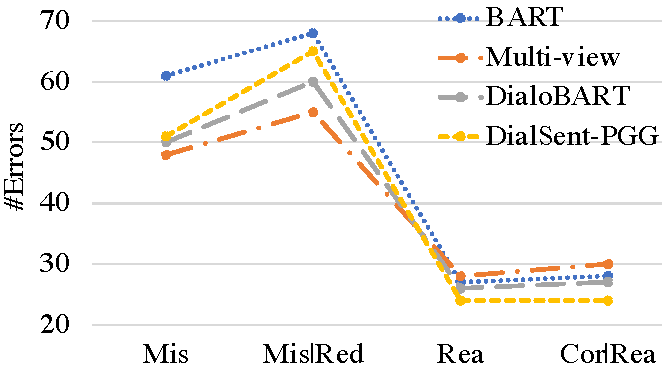
\includegraphics[scale=0.4]{humaneval.pdf}
	\caption{Error analysis on SAMSum. }
	\label{fig:humaneval}
\end{figure}
For error analysis, the Fleiss Kappa for Mis, Red, Cor and Rea are 
$0.55$, $0.10$, $0.26$, $0.42$ respectively. The agreement on Red is 
lower because identifying unimportant information is hard. 
The agreement on Cor is fair due to undistinguishable errors. For example, mismatching of a person and an event among multiple utterances can be either a Cor or a Rea. Besides, Red always leads to Mis. So, 
we divide the error types into two groups and merge them with "OR" logical operation within each group. The Fleiss Kappa for Mis|Red and Cor|Rea are $0.45$ and $0.46$.
We show error types with the agreement larger than $0.40$ in Figure~\ref{fig:humaneval}. 

Multi-view performs better on content selection and 
DialSent-PGG performs better on reasoning and coreference understanding, 
while DialoBART lies in between. 
Fewer errors on Rea and Cor|Rea reflect that our approach 
successfully narrows the understanding gap.
Because references are not the only good summary, high missing content 
doesn't mean that the generated summary is unacceptable. 
As a result, the model with fewer Cor|Rea errors receives higher overall score.

%\begin{table}
%	\small
%	\centering
%	\begin{tabular}{lcccccc}
%		\toprule[1pt]
%		\textbf{} & \textbf{Mis}& \textbf{Red} & \textbf{M|R}&\textbf{Cor} &  \textbf{Rea} & \textbf{C|R\'}\\
%		\midrule[1pt]
%		{BART} & 61 & 20&68 & 14&27& 43\\
%		{Multi-view} &48 &23& 66& 17& 28&30\\
%		{DialoBART} &  50 &19&60& 13&26&27\\
%		{DialSent-PGG} &51& 21&65&16 &24&24\\
%		\bottomrule[1pt]
%	\end{tabular}
%	\caption{Human evaluation results on SAMSum.}
%	\label{tab:end2endhuman}
%\end{table}


\textbf{Implementation Costs:} 
We compare the implementation costs between our approach and two state-of-the-art models, i.e. Multi-view and DialoBART, in Table~\ref{tab:end2endcost}
Although explicitly injecting features for dialogue understanding is effective, labels for these features are hard to collect and implementation costs for these approaches on a new dataset are high. 
Multi-view and DialoBART proposed doing labeling automatically with unsupervised algorithms or language models. However, these labeling approaches bring extra hyper-parameters which are different between datasets and need to be found by trial and error. If we use the same keywords extraction ratio, similarity threshold and topic segmentation ratio from SAMSum directly, the results on DialSumm are only 50.61/26.67/49.06 (Rouge-1/2/L). We searched for the best combination of hyper-parameters following their paper and did 14 trials, while applying our approach on DialSumm only need 4 trials.
%%, DialSent-PGG is trained for 29,908 steps including post-training and fine-tuning for all of the trails, while DialSumm is trained for 41,406 steps.

On the other hand, injecting features increases the requirement of GPU memory. 
With the same training parameters(max tokens$=$1024, batch size$=$1, gradient checkpointing$=$False), Multi-view with double-encoder design encounters an out-of-memory error on RTX 2080Ti with 11G GPU memory. DialoBART occupies around 10.36G since it lengthens the dialogue with additional annotations. DialSent-PGG only occupies 9.87G during post-training for recording the length of the prefix, and 9.65G during fine-tuning which is the same as vanilla BART.  
In a word, our approach costs less for implementation.

\begin{table}[th]
	\small
	\centering
	\begin{tabular}{lcccc}
		\toprule[1pt]
		\textbf{Models} & \textbf{Mem} & \textbf{\#HP}& \textbf{\#Tri}&\textbf{\#St} \\
		\midrule[1pt]
		{Multi-view} &OOM &5 &- &-\\
		{DialoBART} &10.36G &3 &14 &38.61k\\
		{DialSent-PGG} &9.87G/9.65G&1 &4 & 19.32k\\
		\bottomrule[1pt]
	\end{tabular}
	\caption{The upper-bound of GPU memory footprint (Mem), newly introduced hyper-parameter counts (\#HP), the number of trails (\#Tri) and total training steps (\#St) for implementing different models.}
	\label{tab:end2endcost}
\end{table}
%%9881MB finetune; posttrian: 10109
%10607MB dialoBART
%Multiview: HMM: n_components, n_iter C99:window=4, std_coeff=1 temperature
%DialoGPT: Topic, redundancy, keyword
%our: linguistic

% our:(5+3+6+3)* 701 + (7+3+2+7)*390 = 17*701 + 19*390 = 19327
%29*701+31*309=29908
% dialoBART: (8+5+5+9+7+7+9+6+8+7+6+7+8+7)*390  = 99*390 = 38610
% 134*309 = 41406
